%%%%%%%%%%%%%%%%%%%%%%%%%%%%%%%%%%%%%%%%%%%%%%%%%%%%%%%%%%%%%%%%%%%%
%% I, the copyright holder of this work, release this work into the
%% public domain. This applies worldwide. In some countries this may
%% not be legally possible; if so: I grant anyone the right to use
%% this work for any purpose, without any conditions, unless such
%% conditions are required by law.
%%%%%%%%%%%%%%%%%%%%%%%%%%%%%%%%%%%%%%%%%%%%%%%%%%%%%%%%%%%%%%%%%%%%

\documentclass[
  digital, %% This option enables the default options for the
           %% digital version of a document. Replace with `printed`
           %% to enable the default options for the printed version
           %% of a document.
  table,   %% Causes the coloring of tables. Replace with `notable`
           %% to restore plain tables.
  nolof,     %% Prints the List of Figures. Replace with `nolof` to
           %% hide the List of Figures.
  nolot,     %% Prints the List of Tables. Replace with `nolot` to
           %% hide the List of Tables.
  oneside, %% or twoside
  nocover,
  monochrome,
  12pt
  %% More options are listed in the user guide at
  %% <http://mirrors.ctan.org/macros/latex/contrib/fithesis/guide/mu/fi.pdf>.
]{fithesis3}
%% The following section sets up the locales used in the thesis.


\usepackage[many]{tcolorbox}
\tcbuselibrary{listings}

\newtcblisting{mylisting}{
  listing only,
  hbox,
  colframe=gray,
  colback=gray!10,
  listing options={
    basicstyle=\small\ttfamily,
    breaklines=false,
  	frame=none,
    columns=fullflexible
  }
}

\usepackage{caption}
\usepackage{listings}
\usepackage{color}
\usepackage{float}
\usepackage{fancyvrb}
\usepackage{epsfig}

\renewcommand{\lstlistingname}{Ukázka kódu}
\renewcommand{\lstlistlistingname}{Ukázky kódu}

\definecolor{dkgreen}{rgb}{0,0.6,0}
\definecolor{gray}{rgb}{0.5,0.5,0.5}
\definecolor{mauve}{rgb}{0.58,0,0.82}
\lstset{
  frame=tb,
  language=Java,
  captionpos=b,                    % sets the caption-position to bottom
  aboveskip=3mm,
  belowskip=3mm,
  showstringspaces=false,
  columns=flexible,
  basicstyle={\small\ttfamily},
  numbers=none,
  numberstyle=\tiny\color{gray},
  keywordstyle=\color{blue},
  commentstyle=\color{dkgreen},
  stringstyle=\color{mauve},
  breaklines=true,
  breakatwhitespace=true,
  tabsize=3
}
\usepackage{graphicx}
\usepackage{hyperref}
\usepackage[resetfonts]{cmap} %% We need to load the T2A font encoding
\usepackage[T1,T2A]{fontenc}  %% to use the Cyrillic fonts with Russian texts.
\usepackage[
  main=czech, %% By using `czech` or `slovak` as the main locale
                %% instead of `english`, you can typeset the thesis
                %% in either Czech or Slovak, respectively.
  english, german, russian, slovak %% The additional keys allow
]{babel}        %% foreign texts to be typeset as follows:
%%
%%   \begin{otherlanguage}{german}  ... \end{otherlanguage}
%%   \begin{otherlanguage}{russian} ... \end{otherlanguage}
%%   \begin{otherlanguage}{czech}   ... \end{otherlanguage}
%%   \begin{otherlanguage}{slovak}  ... \end{otherlanguage}
%%
%% For non-Latin scripts, it may be necessary to load additional
%% fonts:
\usepackage{paratype}
\def\textrussian#1{{\usefont{T2A}{PTSerif-TLF}{m}{rm}#1}}
%%
%% The following section sets up the metadata of the thesis.
\thesissetup{
    university    = mu,
    faculty       = fi,
    type          = mgr,
    author        = Bc. Tomáš Skopal,
    gender        = m,
    advisor       = RNDr. Filip Nguyen,
    title         = {Distribuované Komplexní Zpracování Událostí},
    TeXtitle      = {Distribuované Komplexní Zpracování Událostí},
    keywords      = {CEP, Kafka, ZooKeeper, analýza, distribuovaný},
    TeXkeywords   = {CEP, Kafka, ZooKeeper, analýza, distribuovaný},
    date			 =	2016/05/30
}
\thesislong{abstract}{
    Goal of this thesis is to develop a algorithm for distributed Event Pattern matching.. The application should be able to run any number of processing nodes. For the needs of this thesis, example of 4 nodes will be sufficient.
}

%% The following section sets up the bibliography.
\usepackage{csquotes}
\usepackage[              %% When typesetting the bibliography, the
  backend=biber,          %% `numeric` style will be used for the
  style=numeric,          %% entries and the `numeric-comp` style
  citestyle=numeric-comp, %% for the references to the entries. The
  sorting=none,           %% entries will be sorted in cite order.
  sortlocale=auto         %% For more unformation about the available
]{biblatex}               %% `style`s and `citestyles`, see:
%% <http://mirrors.ctan.org/macros/latex/contrib/biblatex/doc/biblatex.pdf>.
\addbibresource{example.bib} %% The bibliograpic database within
                          %% the file `example.bib` will be used.
\usepackage{makeidx}      %% The `makeidx` package contains
\makeindex                %% helper commands for index typesetting.
%% These additional packages are used within the document:
\usepackage{paralist}
\usepackage{amsmath}
\usepackage{amsthm}
\usepackage{amsfonts}
\usepackage{url}
\usepackage{menukeys}
\begin{document}
\chapter{Úvod}

Obecně zadání práce říká, že má být vytvořen middleware pro distribuované zpracování vzorů událostí (angl. middleware solution for distributed event pattern matching). Z anglického popisu vychází zkratka MSFDEPM. Zjednodušením dostaneme "distributed event matching", neboli DEM. Pro účely této práce a snadnější orientaci budu popisované řešení identifikovat zkratkou \textit{DEM}.

TODO - dopsat

\chapter{Zpracování událostí}
Se zvyšujícím se počtem zařízení, která jsou schopna produkovat data, se zvyšuje potřeba tato data analyzovat. Běžně rozšířeným způsobem je zpracování dat dávkově. Tedy, data se uloží a ve vhodnou dobu, typicky v noci, se analyzují.

Pokud však uvažujeme reálný provoz na síti, který se dnes v centrálních uzlech pohybuje okolo $1 Tb/s$
[\ref{bib_celeda}], je dávkové zpracování nereálné. Potřebujeme data analyzovat za běhu (angl. real time).

Jednotkou zpracování dat je událost (angl. event). Událost je základním pojmem používaným v oblasti zpracování událostí. Je definována jako objekt, který reprezentuje záznam o aktivitě v daném systému. Událost může mít vlastnosti. Typickým příkladem takové vlastnosti je čas vzniku události, příčina jejího vzniku nebo její typ [\ref{bib_1}]. Jednoduchým příkladem události může být paket. Je to datová schránka, která obsahuje informace, které můžeme analyzovat. Samostatný paket nemá téměř žádnou vypovídající hodnotu, kdežto proud paketů je základem Internetu.

Takový proud událostí skrývá množství dat, která je možné získat až při komplexní analýze, která zohledňuje více událostí v řadě. To nazýváme \textit{komplexní zpracování dat (angl. complex event processing neboli CEP)}


\section{CEP}

CEP je dynamický vědní obor, který se v poslední době hodně rozvíjí\footnote{Důkazem je aktivní komunita, která diskutuje problematiku na konferencích. Například konference v Oslu v roce 2015 (\url{http://dblp.uni-trier.de/db/conf/debs/debs2015.html})}. David Luckham ve své knize \textit{The Power Of Events: An Introduction To Complex Event Processing In Distributed Enterprise Systems} [\ref{bib_1}] definuje CEP jako soubor technik a nástrojů, které pomáhají k pochopení a kontrole událostmi řízených systémů.

Jak už bylo řečeno, množství událostí v systémech je enormní. Při jejich zpracování se setkáváme s pojmem \textit{komplexní událost}. Taková událost se může vyskytnout pouze jako reakce na sled jiných, dílčích, událostí. Dílčí události mohou spolu souviset mnoha různými způsoby, nejčastěji je však spojujeme na základě vlastností (čas vzniku, příčina vzniku, typ, atd).

Příkladem komplexní události může být akce nakoupení produktu v internetovém obchodě. Je to v dnešní době elektronického marketingu velké téma. Běžnému uživateli Internetu je v mnoha kanálech (Facebook ads, Google ads, mailing) zobrazována reklama. Některý uživatel nakoupí produkt při prvním zobrazení určité reklamy. Jiný uživatel potřebuje reklamu vidět alespoň pětkrát, než nakoupí. Způsob jak tuto "cestu" měřit se jmenuje atribuční model [\ref{bib_6}]. Atribuční model je tak defacto soubor událostí, které vyvolaly konečnou, komplexní, událost. Tedy nákup produktu v obchodě. S roustoucím počtem zařízení, roste počet reklam a také se komplikují atribuční modely. Vhodnými technikami zpracování dílčích událostí (zobrazení reklamy, kliknutí na reklamu, nainstalování aplikace) lze například predikovat chování uživatele.

CEP nabízí techniky pro definici a využití vztahů mezi událostmi. Může být využíván pro analýzu libovolného typu událostí v aplikaci, počítačové síti nebo v informačním systému. Jednou z těchto technik je i definování vlastních událostí, jakožto pravidla. Jinak řečeno, můžeme vytvořit vlastní reakci na soubor určitých událostí v našem systému. Touto cestou můžeme pochopit co se v našem systému odehrává.

To zvyšuje míru flexibility. Uživatel může za pomocí CEP specifikovat taková pravidla, která jej aktuálně zajímají a jsou pro něj přínosem. Může analyzovat jak nízko-úrovňové, tak vysoko-úrovňové procesy. Různé druhy událostí mohou být v CEP monitorovány současně. Velkou výhodou je, že pravidla mohou být měněna, odebírána a přidávána za běhu, tedy bez výpadku systému.

Zpracování proudu událostí a vyhodnocení, jestli se pravidlo vyskytlo, stojí samozřejmě určitý výpočetní výkon. V závislosti na typu a množství dat. Pokud je dat hodně (například analýza síťového provozu), musíme výpočet distribuovat.
 
\section{Distribuované CEP}
Úvodem kapitoly je potřeba jasně vymezit co v tomto kontextu chápeme pod pojmem "distribuovaný". Obecně se používají dva výklady:
\begin{itemize}
  \item Distribuované zpracování událostí jako zpracování událostí z více heterogenních zdrojů (distribuovaný systém).~[\ref{bib_2}] Takový výpočet může běžet i na jenom stroji a samotná analýza většinou nebývá paralelní. Takto pojem používá i \textit{David Luckham} v knize \textit{The Power of Events} [\ref{bib_1}] v popisu obrázku \textit{1.1}.
  \item Distribuované zpracování událostí jako výpočet rozdělený na více menších, méně náročných úloh za účelem rychlejšího zpracování s využitím paralelismu\footnote{Takto zpracovává data například Twitter [\ref{bib_distributed_computing}]. A to jejich distribucí pomocí nástroje \textit{Apache Storm}}. Dále v práci budeme pojem chápat právě takto.
\end{itemize}

Požadavky na distribuované zpracování událostí (DCEP) jsou v mnoha ohledech jiné než na zpracování centralizované. Dvě hlavní vlastnosti, které vyžadujeme jsou vysoká míra dostupnosti (angl. availability) a nízké zpoždění (angl. latency). Cílem je pak maximalizovat dostupnost a minimalizovat zpoždění. Bohužel u většiny návrhů platí, že tyto vlastnosti jsou závislé a zlepšení jedné, zhoršuje druhou. Zlepšení dostupnosti, zvýší zpoždění, protože potřebujeme více času na synchronizaci všech řídících informací. [\ref{bib_3}]

Zmíněné dvě vlastnosti nejsou jediné. Mezi vlastnosti distribuovaného zpracování události můžeme dále zařadit:
\begin{itemize}
  \item rovnoměrné rozdělení dat mezi výpočetní uzly (angl. data partitioning)
  \item automatické škálování výpočtu
  \item tolerance chyb
  \item správa datového úložiště
\end{itemize}

\chapter{Nástroje pro distribuované zpracování událostí}
TODO - dopsat
\section{Apache Samsa}
\section{Apache Storm}
\section{CAVE}
%% http://dl.acm.org/citation.cfm?doid=2675743.2771834
\chapter{Analýza}
\label{sec:analysis}

Tato kapitola popisuje požadavky na systém a zasazuje systém do prostředí ve kterém bude nasazen. Počátek kapitoly parafrázuje a rozvíjí zadání práce. Dále je diagram užití, který shrnuje funkční požadavky. Na konci kapitoly jsou na modelovém příkladě demonstrovány vstupy a výstupy systému.

Cílem této práce je vytvoření software pro distribuované zpracování událostí, který bude schopen detekovat komplexní události na základě pravidel. Aplikace by měla být schopna zvládnout libovolný počet připojených uzlů. Síť propojených uzlů je možné reprezentovat grafem G(V, E), kde V jsou uzly grafu, neboli konkrétní počítače na kterých probíhá zpracování. E jsou pak orientované hrany grafu, které reprezentují informaci o tom který počítač posílá data kterému. Každá hrana je označena příznakem \textit{$L_i$}, který označuje typ události, která je po dané hraně posílána. Konkrétním příkladem tak může být událost \textit{$L_1$}, představující zprávu typu \textit{chyba}, která není tak častá, ale její závažnost je vyšší. A událost \textit{$L_2$}, představující zprávu typu \textit{upozornění}, která je častá, ale méně závažná.

Pravidla pro detekci komplexních událostí, budou mít časovou platnost. Po uplynutí daného času se pravidlo automaticky stane neaktivní. Pravidla bude také možné nasadit pouze na určitou podmnožinu uzlů V grafu G. Více o pravidlech v kapitole \ref{sec:usecase_rule}.

Na obrázku \ref{fig:analysis_case_1} je vidět příklad grafu, kde je na uzlu \textit{$V_1$} nasazeno pravidlo analyzující události \textit{$L_1$}.

\begin{figure}[H]
	\centering
    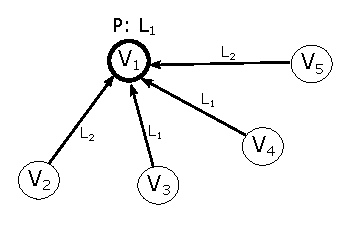
\includegraphics[width=0.4\textwidth, height=0.15\textheight]{images/analysis_case_1.eps}
    \caption{Před vyhodnocením pravidla \textit{P: $L_1$} existuje jeden uzel zpracovávající události}
    \label{fig:analysis_case_1}
\end{figure}

Po určitém počtu výskytů události \textit{$L_1$} je vytvořena nová skupina z uzlů \textit{$V_3$} a \textit{$V_4$} kde je \textit{$V_4$} zvolen hlavním uzlem. Viz obr. \ref{fig:analysis_case_2}

\begin{figure}[H]
	\centering
    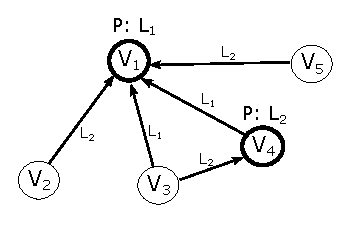
\includegraphics[width=0.4\textwidth, height=0.15\textheight]{images/analysis_case_2.eps}
    \caption{Po vyhodnocení pravidla \textit{P: $L_1$} existují dva uzly zpracovávající události}
    \label{fig:analysis_case_2}
\end{figure}

Typickým místem pro nasazení distribuovaného zpracování událostí je analýza síťové komunikace. To je také místo, kde bude DEM nasazen.

Nejčastější případ, je ten, že přes jeden hlavní uzel probíhá většina komunikace. Podobně je tomu i v softwaru. Aplikační server zpracovává všechny klientské požadavky. Takový uzel je zdrojem dat, která chceme analyzovat. Vytváří sekvenční proud dat, který můžeme vhodně distribuovat do clusteru. Ten jej zpracovává.

Problém nastane, když je množství produkovaných dat větší než je kapacita analyzujícího (analyzujících) počítačů. V takovém případě můžeme přidat výpočetní sílu nebo zvolit úplně jiný přístup k datové analýze.

\section{Vstupy a výstupy}
Uvažujme situaci, kdy necháme na síťovém uzlu aby analyzoval běžně známe hrozby. Taková zařízení jsou na trhu běžně dostupná. A zbytek analýzy bude probíhat až na uzlech v rámci sítě. V modelové situaci útočník obejde firewall a na koncových zařízeních v síti začnou vznikat anomálie. Za normální situace by se takový útok neodhalil, protože na koncových zařízeních neběží žádná detekce. Často to ani není prakticky možné, protože kdyby počítače odesílaly všechen provoz do clusteru na analýzu, byla by to ještě větší zátěž než, kdyby to dělal hlavní síťový prvek. Cílem této práce je tak vytvořit řešení, které bude možno nasadit přímo na koncová zařízení a provádět analýzu tam. Hrubou představu znázorňuje obrázek \ref{fig:cloud-comparison}

\begin{figure}[H]
	\centering
    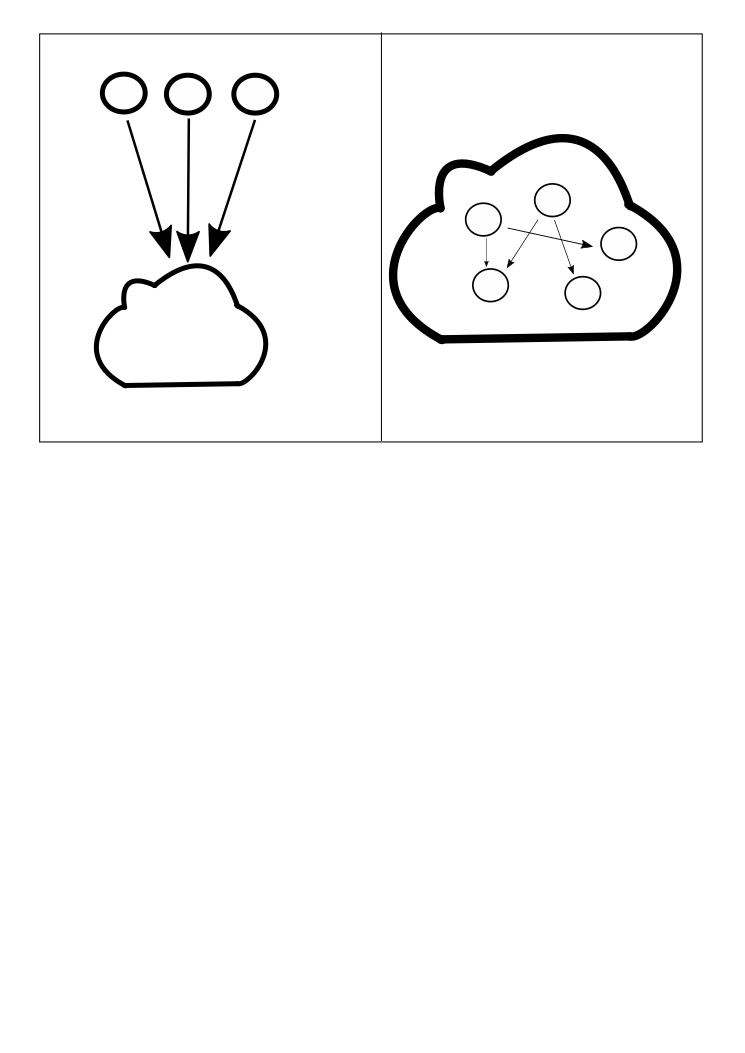
\includegraphics[width=0.4\textwidth, height=0.35\textheight]{images/cloud-comparison.png}
    \caption{Srovnání přístupu zasílání dat do cloudu (v levo) a vytvoření cloudu přímo na koncových zařízeních (v pravo)}
    \label{fig:cloud-comparison}
\end{figure}

Vstupem jsou data zaznamenána na každém stroji připojeném do \textit{DEM}. Formát, množství a povaha dat je pak určena konkrétní situací, která je potřeba sledovat. Pro účely této práce jsou data naivně generována aby vytvořila simulaci síťového útoku. Detailní popis je v kapitole~\ref{sec:udalosti-v-systemu}

Výstupem by mělo být upozornění na nestandardní situaci v části nebo celém systému. Formát výstupu DEM je opět individuální vzhledem k situaci. Zjištěné výsledky mohou být ukládány ve formě logů (tak je to vyřešeno v této práci), odesílána do centrálního dohledu nebo ukládána do databáze.

Do DEM bude možno nasadit pravidla na detekci vzorů událostí. Tato pravidla mohou být omezena časovou platností a nasazena na analýzu pouze určitého množství uzlů.

\section{Diagram užití}
Cílem této kapitoly je jasně formulovat seznam požadavků, které má systém splňovat. Soubor požadavků je znázorněn graficky pomocí diagramu užití. Dále jsou všechny požadavky rozepsány. U některých je popis doplněn o pseudokód\footnote{Pseudokód je psán v angličtině, protože angličtina je obecně uznávaný jazyk pro psaní jakéhokoli kódu.}.

Požadavky jsou kladeny hlavně na variabilitu, možnost nasazení pravidel s časovou platností. Menší důraz je na výkon a proces nasazování.

Na obrázku \ref{fig:usecase} je znázorněn diagram užití, který přehledně shrnuje požadavky na systém. Vystupují v něm dvě role. Uživatel, je zde člověk, který spouští analýzu. Druhou rolí je Algoritmus, který reprezentuje samotný software. Je zde uveden proto, aby bylo zřejmé jaké operace se od systému vyžadují.

\begin{figure}[H]
	\centering
    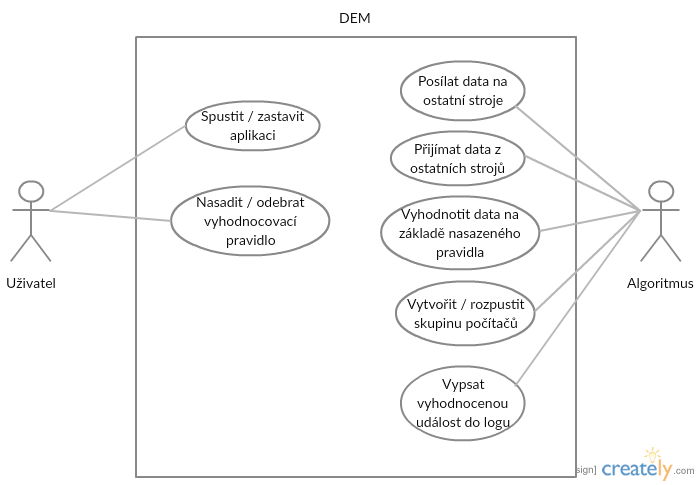
\includegraphics[width=0.9\textwidth, height=0.45\textheight]{images/usecase.png}
    \caption{Diagram užití}
    \label{fig:usecase}
\end{figure}

Dále následuje popis jednotlivých případů užití. Kvůli přehlednosti jsou nadpisy některých pravidel zkráceny.

\subsection*{Spustit / zastavit aplikaci}
Jak je z názvu patrné uživatel může spustit a zastavit aplikaci a s tím samozřejmě i analýzu. Je zde vhodné zdůraznit, že spuštění i zastavení by mělo být centralizované a jednoduché. To znamená kontrola pomocí jednoho skriptu. Tím se ušetří uživateli čas a předejde se některým chybám.

\subsection*{Nasadit / odebrat pravidlo}
\label{sec:usecase_rule}
Uzly, které budou přijímat data, je budou zároveň i analyzovat. Tím, že data mají charakter potenciálně nekonečného proudu, bude pro analýzu potřeba zvolit vhodný nástroj. Nástroj bude muset umět na základě definovaného pravidla vyhodnotit která z příchozích dat pravidlu vyhovují. Jak již bylo zmíněno dat může být opravdu hodně, proto vyhodnocování musí probíhat pouze v omezeném časovém intervalu. Demonstrace pravidla za použití pseudokódu na obrázku \ref{fig:sec_usecase_rule} vyhodnocuje počet událostí typu \textit{$L_1$} v časovém okně pěti sekund.

\begin{center}
\begin{minipage}[H]{\linewidth}
	\begin{mylisting}
SELECT count(*) FROM Event(type='L1') in window (5 sec)
	\end{mylisting}
	\captionof{figure}{Příklad pravidla}
	\label{fig:sec_usecase_rule} 
\end{minipage}
\end{center}

\chapter{Návrh}
Tato kapitola postupně popisuje jak budou reálně splněny požadavky na systém uvedené v analýze. Stěžejní část kapitoly je volba technologií. U každé zvolené technologie je její popis a jak bude použita ve výsledném řešení.

\section{Technologie}
Tato kapitola podkapitola jednotlivé technologie, které jsou použity při implementaci algoritmu. Na konci každé subsekce je popis toho jak konkrétně je technologie použita v mém řešení.

\subsection{Apache Maven}
Apache Maven je nástroj pro správu, řízení a automatizaci sestavování aplikací (angl. build). Maven sám nemá žádné uživatelské rozhraní a běží pouze na příkazové řádce. Jeho účelem je usnadnit práci vývojáři tím, že definuje jednotný proces sestavení. \ref{bib_4} Také definuje strukturu aplikace, protože jednotlivé typy souborů hledá v určitých balíčcích. Například spustitelné Java soubory by měly být v adresáři \textit{src/maven/java}.

Konfigurační soubor Mavenu je \textit{pom.xml}, ve kterém jsou uvedeny zásuvné moduly (pluginy), podle kterých Maven pozná, co má dělat. Také je zde seznam závislostí na externí knihovny, které Maven dokáže stáhnout. Při použití Mavenu je sestavení programu otázkou jen jednoho příkazu (\textit{mvn clean install}).

\subsection*{Použití}
\label{sec:maven-usage}
Kromě definování závislostí je Maven v projektu použit na vytvoření modulů. Moduly jsou celkem čtyři a jsou navrženy tak, aby názvem i logikou odpovídaly účelu a nepřesahovaly své určení. Jsou to:
\begin{itemize}
  \item Producer -- slouží pro generování dat a jejich posílání do Kafky. Data jsou generována v určitých časových intervalech a jejich struktura je přesně daná. Syntax a sémantika vzorových dat je popsána v kapitole \ref{sec:udalosti-v-systemu}. Při reálném použití by byl tento modul přepsán nebo nahrazen za takový, který bude reálná data číst z nějakého systémového nebo aplikačního logu.
  \item Consumer -- tento modul čte data z Kafky a analyzuje je za pomocí nástroje Esper \ref{sec:esper}. Události, které Esper vyhodnotí slouží v DEM jako řídící zprávy pro přechod do dalšího stavu. Případně jsou události pouze zapsány do logu.
  \item MainApp -- modul obsahuje spustitelnou třídu a je tak vstupním bodem programu. Také se zde zpracovávají všechny řídící události ze ZooKeeperu \ref{sec:zookeeper} a rozhoduje se jaká vlákna (konzument nebo producent) se mají vytvořit nebo zastavit.
  \item AppData -- modul obsahuje několik výčtových typů, které jsou společné v celé aplikaci a jednu singleton \footnote{Singleton neboli jedináček je návrhový vzor, který je využívaný, když je potřeba mít pouze jednu instanci dané třídy.} třídu, která drží některá řídící data. Například ip adresu počítače. Tato data mají k dispozici všechny moduly.
\end{itemize}
Protože je veškerá komunikace řízena událostmi a zasíláním zpráv, moduly jsou na sobě relativně nezávislé a v případě potřeby je možné je zaměnit za jiné. 

\subsection{Apache Kafka}
Apache Kafka je systém pro zasílání zpráv. [\ref{bib_5}] Klastr Kafky může být rozdělený mezi několik počítačů, každý nazýváme \textit{broker}. Základem Kafky je fronta zpráv. Ta je reprezentována tématem (angl. topic) respektive přepážkou (angl. partition). Při vytváření tématu udáváme kromě jejího jména, také kolikrát se má replikovat mezi \textit{brokery} a počet přepážek. Přepážka je menší jednotka než téma. Každé téma může být replikováno mezi brokery.

\subsection*{Konzument a producent}

Do kafky data zapisují \textit{producenti} a na druhé straně z ní data čtou \textit{konzumenti} (angl. producer and consumer). Zapisování dat producentem je přímočaré. Producent rozhoduje do kterého tématu či přepážky se má zpráva zapsat. Zprávy jsou ukládány do fronty, tedy způsobem FIFO \footnote{FIFO -- první zapsán, první přečten (angl. first in first out)}. Čtení zpráv závisí na aktuálním stavu. Konzumenty je možné seskupovat do skupin a podle toho se pak rozlišuje způsob čtení zpráv na "queuing" a "publish-subscribe". V modelu "queue" je zpráva poslána vždy jednomu z konzumentů. Naopak v modelu "publish-subscribe" je každá zpráva poslána všem konzumentům. V dokumentaci Kafky se říká [\ref{bib_5}]:
\begin{itemize}
  \item Pokud jsou všichni konzumenti ve stejné skupině, pak Kafka funguje v modelu "queue".
  \item Pokud je každý konzument v jiné skupině, pak je Kafka v modelu "publish-subscribe". Všechny zprávy jsou distribuovány všem konzumentům \footnote{Broadcast}.
\end{itemize}

\begin{figure}[H]
	\centering
    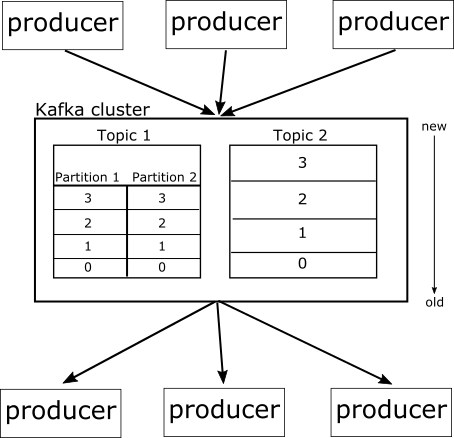
\includegraphics[width=0.65\textwidth, height=0.45\textheight]{images/kafka.png}
    \caption{Znázornění základního schématu Kafky}
    \label{fig:kafka}
\end{figure}

\subsection*{Garance}
Kafka poskytuje následující seznam garancí:
\begin{itemize}
  \item Zprávy poslané do určitého tématu budou seřazeny v pořadí v jakém byly odeslány. Například pokud je zpráva \textit{M1} odeslána producentem dříve než zpráva \textit{M2}, pak Kafka zaručuje, že bude mít zpráva \textit{M1} menší offset a bude v logu zobrazena dříve než \textit{M2}.
  \item Konzument vidí zprávy v takovém pořadí, v jakém byly uloženy do logu.
  \item Pro téma s faktorem replikování \textit{N} (bude replikováno mezi \textit{N} brokerů), Kafka zaručuje zachování dat až pro \textit{N-1} vypadlých serverů.
\end{itemize}

\subsection*{Použití}
Jak už bylo řečeno dříve analýza událostí bude probíhat na počítačích, které data produkují. V navrhovaném řešení jsem nezaznamenal potřebu dělit témata na příčky (partition). Také Kafka není distribuovaná do několika brokerů a je spuštěna pouze na jenom stroji. Distribuci bych nakonfiguroval až v případě produkčního nasazení pro prevenci výpadků. Na každém počítači běží nejméně jeden producent a nejvýše jeden konzument. Jednotlivá témata jsou pojmenována podle ip adres počítačů. Konkrétně při iniciálním spuštění je jeden ze strojů určen jako konzument a počet producentů je roven počtu strojů. Protože existuje pouze jeden konzument, data jsou posílána pouze do jednoho odpovídajícího tématu. Viz obrázek \ref{fig:kafka-impl}

\begin{figure}[H]
	\centering
    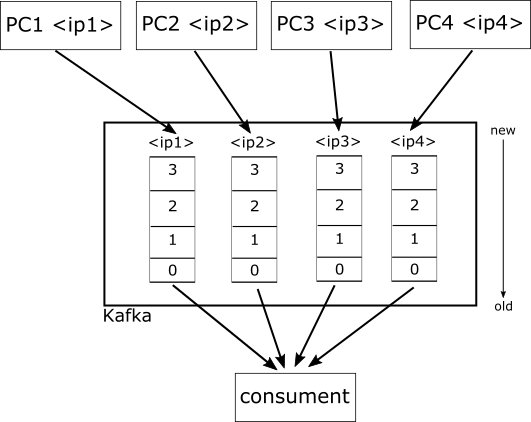
\includegraphics[width=0.55\textwidth, height=0.3\textheight]{images/kafka-impl.png}
    \caption{Struktura Kafky při iniciálním spuštění}
    \label{fig:kafka-impl}
\end{figure}

\newpage
\subsection{Apache ZooKeeper}
\label{sec:zookeeper}
ZooKeeper je další z rodiny "open-source" Apache technologií. Je to centralizovaná služba pro správu konfiguračních dat, pojmenování a poskytování synchronizace distribuovaných uzlů. [\ref{bib_7}]

ZooKeeper je navržen, tak aby jej bylo jednoduché použít. Je napsán v Javě a poskytuje konektory pro Javu a pro C. Struktura datového modelu je podobná stromovému uspořádání souborového systému. Datový model ZooKeeperu je sestaven z uzlů zvaných \textit{znodes}. Na rozdíl od klasického souborového systému, který je navržen pro dlouhodobé ukládání dat, ZooKeeper data drží v paměti, a tak může dosahovat nízkého zpoždění a vysoké propustnosti. Pro ilustraci, uvažujme jednoduchý příklad: Každý znode může obsahovat data (až do limitu 1MB). V takovém případě znode reprezentuje soubor (řekněme textový) v souborovém systému. V ZooKeeperu může mít každý uzel nula až N potomků. Pak znode vystupuje obdobně jako složka v souborovém systému. Každý znode může zároveň obsahovat data a mít potomky.

\subsection*{Garance}
Obdobně jako Kafka a naprostá většina distribuovaných systémů, musí i ZooKeeper poskytovat určité garance běhu v distribuovaném prostředí.

\begin{itemize}
  \item Sekvenční konzistence -- změny na uzlu jsou aplikovány v takovém pořadí v jakém byly odeslány (modifikace dat, odebrání nebo přidání potomka, apod).
  \item Atomicita -- změny jsou úspěšně aplikovány úplně nebo neprovedeny vůbec. Neexistuje žádný mezistav.
  \item Spolehlivost -- Jakmile je změna aplikována, je stav uzlu garantován. Nemění se až do doby další změny.
  \item Časová konzistence -- Stav systému je po uplynutí definovaného času vždy aktuální.
\end{itemize}

\subsection*{API}
ZooKeeper nabízí uživateli (programátorovi) velice jednoduché rozhraní, pro manipulaci s jednotlivými uzly. Sestává se z těchto operací:
\begin{itemize}
  \item Vytvoření (create)
  \item Smazání (delete)
  \item Kontrola existence uzlu (exists)
  \item Získání dat (get data)
  \item Zapsání dat (set data)
  \item Získání všech potomků daného uzlu (get children)
  \item Ukazatel dokončení synchronizace dat (sync)
\end{itemize}

Kromě operace \textit{sync} jsou v této práci použity všechny.

\subsection*{Pozorovatelé}
Pozorovatelé \footnote{Z anglického slova \textit{Watches}. Jde o konkrétní implementaci návrhového vzoru "observable". [\ref{bib_8}]} jsou nedílnou součástí téměř každého událostmi řízeného systému. Stejně tak, je tomu u ZooKeeperu. Na znode je možné zaregistrovat dva druhy pozorovatelů:

\begin{itemize}
  \item Datový pozorovatel -- změní stav, když jsou změněna data v uzlu. Tzn někdo zavolal operaci "zapsání dat". Změna stavu obsahuje nově nastavená data
  \item Pozorovatel potomků -- změní stav, když nastane změna v některém z potomků daného uzlu. Událost obsahuje, mimo jiné, informaci o typu změny (smazání, vytvoření, zápis dat, ztráta konektivity) a identifikaci potomka. 
\end{itemize}

\subsection*{Apache Curator}
Aplikační rámec \textit{Curator}	je nástroj vytvořený společností Neflix pro jednodušší práci se ZooKeeperem. Rozhraní ZooKeeperu se potýká s několika problémy, jako je například nedostatečné ošetření výpadků konektivity nebo selhání operace. Proto byl navržen \textit{Curator}, který se osvědčil a později přešel pod licenci \textit{Apache}. Poskytuje následující benefity:

\begin{itemize}
  \item Komplexnější rozhraní pro jednodušší práci se ZooKeeperem. \ref{code:curator}
  \item Automatické připojení na instanci ZooKeeperu a automatické opravy výpadků.
  \item Kompletní a dobře otestovaná implementace některých složitějších operací.
\end{itemize}

\begin{lstlisting}[label=code:curator,caption={Demonstrace jednoduchého použití aplikačního rámce Curator, na smazání uzlu \textit{zkNode1} a všech jeho potomků.},language=Java]
curatorFramework.delete()
   .guaranteed()
   .deletingChildrenIfNeeded()
   .forPath("/zkNode1");
\end{lstlisting}

 
\subsection*{Použití}
ZooKeeper je použit pro řízení běhu celého procesu DEM. Jeho hlavní úlohou je distribuce řídících dat mezi jednotlivými výpočetními jednotkami. Druhou funkcí, která logicky vychází ze stromové struktury datového modelu, je reflexe aktuálního stavu aplikace.

Je důležité zmínit, že cesta ve stromové struktuře je určena jednoznačným textovým identifikátorem. Jednotlivé uzly jsou pak odděleny lomítkem. Na obrázku \ref{fig:zookeeper-impl} můžeme vidět strukturu uzlů, při iniciálním spuštění DEM. Příklad identifikátoru prvního uzlu z druhé vrstvy je \textit{"/root/ip1/ip1"}, druhého uzlu z první vrstvy \textit{"/root/ip2"}, atd.

Obrázek \ref{fig:zookeeper-impl} dále znázorňuje logickou strukturu DEM. První vrstva reprezentuje konzumenty a druhá vrstva producenty. Jinak řečeno "kdo komu posílá data". Podstatné je, uvědomit si, že strom zobrazuje pouze virtuální stav. Aplikace jako taková běží na daném stroji vždy jen jednou a strom pak reprezentuje spíše množství běžících vláken a jejich úlohu. Jak je vidět z obrázku \ref{fig:zookeeper-impl}, v DEM existují 4 producenti (jeden na každém fyzickém stroji) a jeden konzument (fyzický stroj s \textit{ip1}). To odpovídá stavu Kafky z obrázku \ref{fig:kafka-impl}.

Výhody stromové struktury jsou zřejmé. U každého uzlu se dá zjistit jaké má potomky (které stroje posílají data a kam). Změna cíle, kam má stroj posílat data, je na úrovni rozhraní triviální. Stačí přesunout uzel v druhé vrstvě pod jiného rodiče.

\begin{figure}[H]
	\centering
    
\includegraphics[width=1\textwidth, height=0.22\textheight]{images/zookeeper-impl.png}
    \caption{Stromová struktura uzlů v Zookeeperu při iniciálním spuštění.}
    \label{fig:zookeeper-impl}
\end{figure}

\subsection{Esper}
\label{sec:esper}
TODO - dopsat

\subsection*{Použití}
%% je potřeba detailne rozebrat jedno konkretni pravidlo, ktere pouzivam a vysvetlit jednotlive casti

\section{Shrnutí}
Kapitola obsahuje přehlednou tabulku, která konkrétně ukazuje která technologie je použita při implementaci daného požadavku z analýzy. A návrh schématu. Schéma je znázorněno na čtyřech strojích.

\begin{table}[H]
  \centering
  \begin{tabularx}{\textwidth}{lllX}
    \toprule
    Požadavek & Technologie \\
    \midrule
    Posílání zpráv mezi stroji & Kafka \\
    Libovolný počet připojených uzlů & ZooKeeper + Kafka \\
    Nasazení nového pravidla & ZooKeeper \\
    Definování chování jednotlivých strojů & ZooKeeper \\
    Vytvořit nebo rozpustit skupinu strojů & ZooKeeper \\
    Nalezení určitého vzoru (pattern) v datech & Esper \\
    Propojit technologie do funkčního celku & Java + Maven \\
    \bottomrule
  \end{tabularx}
  \caption{Splnění požadavků na systém}
  \label{tab:fulfill-usecases}
\end{table}

\begin{figure}[H]
	\centering
    
\includegraphics[width=.7\linewidth, height=.57\textheight]{images/app-architecture.png}
    \caption{Schéma aplikace, které znázorňuje které technologie jsou nasazeny na každém stroji a jaké mají mezi sebou vazby.}
    \label{fig:app-architecture}
\end{figure}

\section{Události v systému}
\label{sec:udalosti-v-systemu}
Povaha a struktura vyhodnocovaných dat je neopomenutelnou součástí každého systému, tedy i tohoto. Pro potřeby analýzy zavedeme dva druhy událostí, \textbf{hrubozrné} a \textbf{jemnozrné}. Hrubozrné jsou události, které nenastávají příliš často, ale mají v systému důležitý význam. Jemnozrné naopak.

Jak je nastíněno v kapitole \label{sec:analysis}, budeme se zabývat analýzou síťové komunikace. Základem je zde samozřejmě proud paketů. Příchozí pakety mohou mimo jiné znamenat pro daný stoj bezpečnostní hrozbu. Například při útoku \textit{SYN flood} je restart (kolaps) stroje způsoben zahlcením pakety s příznakem \textit{SYN}. Zde můžeme za hrubozrnou událost považovat signalizaci restartu stroje. Jemnozrné události jsou pak jednotlivé pakety.

Principem analýzy je identifikace strojů s výskytem stejných hrubozrných událostí a pustit na nich analýzu jemnozrných událostí, která ma za cíl odhalit příčinu.
 
\subsection*{Hrubozrnné}
Hrubozrné události mají komplexní povahu. Jsou tedy výsledkem nějakého složitějšího procesu. Ve výše uvedeném příkladě šlo o restart počítače způsobený cíleným útokem. Jiným příkladem může být chybová zpráva v aplikaci (angl. error log). Pokud je aplikace zasažena \textit{DoS} útokem, pak je hrubozrnou událostí její nedostupnost. V DEM jsou hrubozrné události reprezentovány štítkem \textbf{LEVEL1}.
 
\subsection*{Jemnozrnné}
Tento druh událostí se vyskytuje běžně a sama o sobě nemá událost prakticky žádný význam. Například jeden paket s s příznakem \textit{SYN} se v síťové komunikaci objevuje běžně. V DEM jsou hrubozrné události reprezentovány štítkem \textbf{LEVEL2}.

\chapter{Nasazení}
Předchozí kapitoly Analýza a Návrh shrnují požadavky na systém a technologie, za pomoci kterých budou požadavky splněny. V Návrhu je také popsáno jak bude konkrétně daná technologie použita. Tato kapitola navazuje samotnou implementací a testováním. Je zde popsán běh programu od úplného začátku, tedy správné konfigurace, až po ukázky výstupu. 

\section{Konfigurace}
Jak Kafka, tak ZooKeeper nabízejí velkou variabilitu v konfiguraci. Oficiální dokumentace obou technologií obsahují dobrý popis konfigurace. Proto je tato kapitola věnována pouze konkrétním ukázkám konfigurací v DEM.

Pro spuštění Kafky je důležitý soubor \textit{server.properties}. Obsahuje množství atributů, které se dají modifikovat. Většinu z nich není potřeba upravovat. Měnil jsem pouze \textit{broker id}, \textit{název stroje (host name)} a \textit{seznam ZooKeeper instancí}. Výňatek z konfiguračního souboru s upravenými hodnotami je na obrázku \ref{fig:kafka-conf}.

\begin{center}
\begin{minipage}[H]{\linewidth}
	\begin{mylisting}
broker.id=0
host.name=147.251.43.181
zookeeper.connect=147.251.43.181:2181,147.251.43.130:2181
	\end{mylisting}
	\captionof{figure}{Výňatek z konfiguračního souboru Kafky}
	\label{fig:kafka-conf} 
\end{minipage}
\end{center}

U ZooKeeperu je potřeba upravit dva konfigurační soubory. První je \textit{zoo.cfg}. V něm se nastavují ip adresy a porty ostatních ZooKeeper instancí. Také se nastaví složka do které se ukládají dočasné soubory a je zde i druhý z konfiguračních souborů \textit{myid}. Soubor \textit{myid} obsahuje pouze jedno číslo, které jednoznačně identifikuje instanci a musí být unikátní.

\begin{center}
\begin{minipage}[H]{\linewidth}
	\begin{mylisting}
# the port at which the clients will connect
clientPort=2181

dataDir=~/data/zookeeper

# specify all zookeeper servers
# The fist port is used by followers to connect to the leader
# The second one is used for leader election
server.1=147.251.43.181:2888:3888
server.2=147.251.43.130:2888:3888
server.3=147.251.43.150:2888:3888
server.4=147.251.43.138:2888:3888
	\end{mylisting}
	\captionof{figure}{Ukázka konfiguračního souboru ZooKeeperu}
	\label{fig:zk-conf} 
\end{minipage}
\end{center}

Na konec pouze krátce uvedu hardwarovou konfiguraci virtuálních strojů na kterých probíhalo testování:

\begin{center}
\begin{minipage}[H]{.5\linewidth}
	\begin{mylisting}
OS: Ubuntu 12.04 x86_64
RAM: 1GB
Procesor: 1 core x86_64
HDD: 20GB
	\end{mylisting}
	\captionof{figure}{Konfigurace virtuálních strojů}
	\label{fig:virt-hw-conf} 
\end{minipage}
\end{center}

\section{Implementace}
\label{sec:implementation}
Pro implementaci byla zvolena Java (konkrétně ve verzi 1.8), protože všechny použité technologie mají dobrá API pro Javu a většina příkladů je právě v Javě. Dalším důvodem je také to, že Java se dobře hodí pro běh aplikací tohoto druhu, protože má dobrou práci s vlákny. Posledním, méně důležitým, důvodem je popularita Javy a snadná čitelnost kódu.

Aplikace je z pohledu počtu řádků poměrně malá, ale je kompletně řízena událostmi. Posílání zpráv v Kafce je asynchronní a ZooKeeper i Esper jsou ze své podstaty událostmi řízené aplikační rámce (angl. frameworky). Proto je architektura pro přehlednost členěna do logických modulů. Jednotlivé moduly jsou podrobně popsány v kapitole \ref{sec:maven-usage}.

Implementace probíhala iterativním vývojem. Nejdříve bylo potřeba nastudovat technologie a zvolit vhodnou konfiguraci. Dále jsem vyzkoušel jednoduchou implementaci základního API Kafky a posílání zpráv na jenom stroji. Dalším logickým krokem bylo vyzkoušet komunikaci mezi dvěma různými počítači v síti. V tomto bodě jsem mohl přidat vyhodnocení vzorů událostí pomocí Esperu.

Aplikace byla tedy nachystána na přidání více počítačů a testování distribuovaného chování. Napsal jsem několik skriptů pro automatizaci vývoje. Skripty jsou součástí práce jako elektronická příloha. Když aplikace zvládala posílání zpráv mezi čtyřmi testovacími stroji mohl jsem začít pracovat na poslední a nejsložitější iteraci. Tou byla integrace ZooKeeperu. Na základě vyhodnoceného vzoru událostí ZooKeeper automaticky sdružuje počítače do pracovních skupin. Skupiny také ruší a umožňuje nasazení nových pravidel pro analýzu.

ZooKeeper je jádrem algoritmu. Na každém uzlu je navěšen posluchač, který zaznamenává změny dat. Aplikace je řízena tím, že je do příslušného uzlu vložen nový datový objekt, který obsahuje akci a příslušná data. Například akce \textit{CREATE} znamená vytvoření nového vlákna, které bude reprezentovat konzumenta dat nebo datového producenta. Ukázka datového objektu je na obrázku \ref{fig:json-example}.

\begin{center}
\begin{minipage}[H]{.8\linewidth}
\centering
	\begin{mylisting}
{
	action: "CREATE",
	mode: "producer",
	level: "LEVEL1",
	parent: "<ip>",
	path: "<zk-path>"
}
	\end{mylisting}
	\captionof{figure}{Ukázka datového objektu pro akci \textit{CREATE} při vytváření producenta}
	\label{fig:json-example} 
\end{minipage}
\end{center}

Seznam hlavních řídících akcí pro ZooKeeper:

\begin{itemize}
  \item CREATE -- vytváří nové vlákno s producentem nebo konzumentem
  \item CREATE\_CHILDREN\_PRODUCER -- pro daný uzel vytvoří úplně nového potomka a spustí v něm vlákno s producentem
  \item STOP\_PRODUCER -- zastaví producenta (stopne a zabije vlákno)
  \item STOP\_CONSUMER -- zastaví konzumenta (stopne a zabije vlákno)
  \item SET\_EP\_RULE -- nastaví v uzlu nové pravidlo pro analýzu
  \item DELETEd\_SELF -- smaže sama sebe (ZooKeeper uzel) včetně zabití všech konzumentů a producentů, které v rámci daného uzlu běží
\end{itemize}

\subsection{Spuštění}
Před spuštěním algoritmu, tedy analýzy dat, je potřeba nastartovat Kafku. Záleží na počtu replikací Kafky. V našem případě je Kafka pouze jako jedna instance. Kafka běží přímo na jednom ze strojů. Dále na každém stroji spustíme ZooKeeper. ZooKeeper potřebuje ke správnému fungování, aby bylo online více než n/2 uzlů, kde n je celkový počet uzlů, které jsou v clusteru. V této práci probíhá testování na čtyřech strojích, tedy pro ZooKeeper musí být online nejméně tři. Jakmile jsou spuštěny tři stroje, ZooKeeper zvolí řídící instanci.

Při spuštění samotné Java aplikace je potřeba zadat několik vstupních parametrů:

\begin{itemize}
  \item \textbf{ip}  -- ip adresa stroje. Slouží také jako jednoznačný identifikátor v ZooKeeperu
  \item \textbf{zklist} -- seznam adres, kde běží jednotlivé instance ZooKeeperu. Prvky v seznamu jsou odděleny čárkou (bez mezery). List potřebuje aplikační rámec Curator [\ref{bib_9}] pro připojení k ZooKeeperu.
  \item \textbf{m} -- označuje mód ve kterém je aplikace spuštěna. Jsou možné dva módy:
  \begin{itemize}
  	\item[*] \textbf{producer} -- aplikace je spuštěna jako producent. To znamená, že se zapojí do ZooKeeper stromu, zaregistruje příslušné posluchače a začne posílat data do Kafky. Do tématu, pojmenovaného podle ip adresy.
  	\item[*] \textbf{combined} -- aplikace je spuštěna jako producent i konzument. Kromě producenta je vytvořen i konzument, který přijímá data z Kafky z tématu podle ip adresy. Data předává na analýzu Esperu.
  \end{itemize}
\end{itemize}

V aplikaci je nastaveno výchozí pravidlo, podle kterého se mají data analyzovat. Jakmile je aplikace úspěšně spuštěna, začne produkovat, případně i konzumovat a analyzovat data. Spuštění každé jedné aplikace znamená, že se v ZooKeeperu vytvoří dva nové uzly, tak jak je vidět na obrázku  \ref{fig:app-start}. Postupně se buduje strom až do finálního stavu, který je vidět na obrázku \ref{fig:zookeeper-impl}.

\begin{figure}[H]
	\centering
    
\includegraphics[width=.4\linewidth, height=.18\textheight]{images/app-start.png}
    \caption{Postupné přidávání uzlů do ZooKeeper stromu}
    \label{fig:app-start}
\end{figure}

\subsection{Přechody mezi stavy}
V předchozí kapitole jsem rozvedl jak probíhá spuštění aplikace do jakého stavu se po spuštění dostane. Tato kapitola se bude podrobněji věnovat tomu, v jakých stavech se může DEM nacházet. Schválně zde zmiňuji DEM, protože předchozí kapitola se věnovala hlavně spuštění z pohledu jedné instance. Zde jsou naproti tomu popsány stavy více z globálního pohledu.

Jakmile je spuštěn konzument, automaticky všechny události předává do Esperu, který je vyhodnocuje. Uvažujme pravidlo, které detekuje příchozích pěti událostí během tří sekund. Každý z počítačů svou aktivitou toto kritérium splní. Jakmile Esper detekuje splnění pravidla, vytvoří událost. Událost je v aplikaci zpracována. Pokud je aktivní jen jeden počítač, nemá smysl spouštět detailní analýzu. Naopak v případě, že vyhodnocení pravidla způsobilo více počítačů, je žádoucí na této podmnožině spustit detailní analýzu.

Přechod do nového stavu začíná volbou nového konzumenta. Tedy počítače, který bude analyzovat proud jemnozrných událostí. Pro volbu jsem zvolil postup, kdy je nalezen první takový počítač, který ještě neprovádí žádnou analýzu. Díky zvolené ZooKeeper struktuře je to jednoduché. Stačí projít první úroveň a hledat uzel, který ještě nemá žádné potomky. Takovému uzlu je nejdříve poslána akce \textit{CREATE}\footnote{Řídící akce ze seznamu z kapitoly \ref{sec:implementation}}, aby spustil vlákno s konzumentem. Pak tolik akcí \\ \textit{CREATE\_CHILDREN\_PRODUCER}, kolik strojů je určených k jemnozrné analýze. Samozřejmě součástí každé akce jsou i potřebná data (ip adresa počítače apod.).

Na obrázku \ref{fig:zookeeper-state-1} je vidět příklad, kdy byly pro jemnozrnou analýzu vybrány stroje \textit{ip1} a  \textit{ip2}. Jak je vidět hrubozrná analýza stále probíhá na stroji \textit{ip1}, proto musí být jako konzument jemnozrných událostí zvolen stroj \textit{ip2}.

\begin{figure}[H]
	\centering
    
\includegraphics[width=.6\linewidth, height=.2\textheight]{images/zookeeper-state-1.png}
    \caption{Ukázka ZooKeeper stromu při současné analýze jemnozrných a hrubozrných událostí}
    \label{fig:zookeeper-state-1}
\end{figure}

Jak už bylo řečeno dříve, ZooKeeper reprezentuje logickou strukturu. Na obrázku \ref{fig:kafka-state-1} je znázorněn odpovídající stav v Kafce. Protože už existují dva konzumenti, jsou v Kafce zaregistrována dvě témata.

\begin{figure}[H]
	\centering
    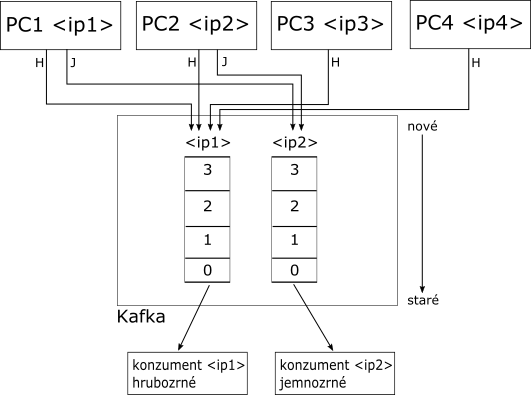
\includegraphics[width=.5\linewidth, height=.3\textheight]{images/kafka-state-1.png}
    \caption{Ukázka stavu Kafky při současné analýze jemnozrných a hrubozrných událostí. Zkratky \textit{J} a \textit{H} na obrázku znamenají jemnozrné a hrubozrné události.}
    \label{fig:kafka-state-1}
\end{figure}

V aktuálním stavu se tedy zároveň analyzují hrubozrné i jmenozrné události. Cílem další hrubozrné analýzy je odhalit jestli danému pravidlu neodpovídají ještě další počítače. Samozřejmě, pokud bude v průběhu jemnozrné analýzy vyhodnocen stejný vzor (stejná sada počítačů), pak se znovu jemnozrná analýza nespouští. Cílem jemnozrné analýzy je odhalit příčinu vzniku nestandardní situace. Logicky jsou tedy na uzlech \textit{ip1} a  \textit{ip2} nasazena jiná pravidla detekující vzory událostí.

Jak jemnozrná, tak hrubozrná pravidla jsou omezena časovou platností. Po uplynutí této doby je hrubozrná analýza zastavena a DEM čeká na nasazení jiného (nebo stejného) pravidla. V případě jemnozrné analýzy je celá práce ukončena a je potřeba "uklidit". To znamená zastavit vlákna s producenty i konzumentem a smazat příslušné uzly v "druhé vrstvě" ZooKeeper stromu. Tak aby se DEM dostal do stavu z obrázku \ref{fig:zookeeper-impl}.

Do uzlu, který zpracovává hrubozrné události je možné kdykoli nasadit nové pravidlo pro detekci vzorů událostí.

\section{Testování}

Kapitola Testování se věnuje ukázkám datových objektů, které byly použity při testování funkčnosti algoritmu. Také jsou zde popsána pravidla, která byla použita pro analýzu. Data neodpovídají reálným, ale jsou vymyšlena aby simulovala určité situace, které jsou postaveny na reálných základech.

Protože bylo z počátku složité uchopit celou myšlenku, začal jsem testovat algoritmus po jednotlivých akcích\footnote{Řídící akce z kapitoly \ref{sec:implementation}}. Pravidlo pro detekci bylo jednoduché a rozlišovalo pouze události úrovně jedna a dvě. Data byla generována na každém stroji v náhodných intervalech \textit{<0.5s - 1s>}. Ukázka datového objektu je na obrázku \ref{fig:data-example-1}.

\begin{center}
\begin{minipage}[H]{.5\linewidth}
	\begin{mylisting}
{
	level: "LEVEL1 / LEVEL2",
	source: <zk-path>
}
	\end{mylisting}
	\captionof{figure}{Ukázka datového objektu z první fáze testování}
	\label{fig:data-example-1} 
\end{minipage}
\end{center}

V této fázi bylo hlavním cílem zjistit jestli Esper správně detekuje vzor událostí. S velkými problémy jsem se setkal při vytváření uzlů v ZooKeeperu. Někdy se uzly vytvářely duplicitně, někdy se vytvořily pod špatným rodičem. Nějakou dobu také trvalo zvolit správný postup vytváření a rušení vláken konzumentů a producentů aby nic nezůstalo "viset v paměti". Jeden příklad za všechny: Když je na uzel v ZooKeeperu navěšen nějaký posluchač a uzel je smazán, neznamená to, že se posluchač stane neaktivním a zruší se. Je ho potřeba explicitně vyjmout z kolekce a až potom smazat uzel. Jinak vznikají duplicity v posluchačích a akce jsou vyhodnoceny vícekrát.

Jakmile byly vyřešeny problémy při jednotlivých akcích, bylo potřeba vymyslet reálnější datový model, který bude ukazovat myšlenku hrubozrné a jemnozrné analýzy. Proto jsem datový objekt rozšířil o další vlastnosti. Viz obrázek \ref{fig:data-example-2}. Myšlenka analýzy je tedy taková, že v akcích úrovně jedna se hledá vzor, který by nasvědčoval útoku. Pokud je takový vzor nalezen, je nad podezřelými počítači spuštěna detailní (jemnozrná analýza). Ta spočívá v počítání všech událostí úrovně dva. Pokud jejich počet v určitém časovém okně přesáhne daný limit, je "útok" prohlášen za reálný a zpráva je zapsána do logu.

\begin{center}
\begin{minipage}[H]{.65\linewidth}
	\begin{mylisting}
{
	level: "LEVEL1 / LEVEL2",
	source: <zk-path>,
	msg: "info textual message",
	flag: "SYN",
	size: 10,
	port: 80
}
	\end{mylisting}
	\captionof{figure}{Ukázka datového objektu z první fáze testování, kde flag reprezentuje příznak v datagramu (SYN a ACK), size velikost paketu a port je cílový port v komunikaci.}
	\label{fig:data-example-2} 
\end{minipage}
\end{center}

\subsection*{Esper pravidla}
Z datového objektu na obrázku \ref{fig:data-example-2} jsou pro nás nyní důležité atributy \menu{flag}, \menu{size} a \menu{port}. Na obrázku \ref{fig:pc-data-distribution} je vidět jak počítače generují testovací data. Neboli distribuce generovaných dat, které reprezentují potenciální hrozbu, mezi počítači.

\begin{figure}[H]
	\centering
    
\includegraphics[width=.65\linewidth, height=.2\textheight]{images/pc-data-distribution.png}
    \caption{Znázornění které počítače v testovacím prostředí produkují kritické typy datových objektů. Zbylé dva atributy jsou u každého počítače nastaveny na "neutrální" hodnotu.}
    \label{fig:pc-data-distribution}
\end{figure}

Data u jednotlivých útoků jsou založena na skutečné podstatě, i když jde spíše o princip. Ve skutečnosti bývají síťové útoky velmi komplikované. Například určitě neplatí, že série dotazů na port číslo 11, automaticky znamená útok skenováním portů. Data jsou primárně zvolena pro demonstraci funkčnosti algoritmu.

Na jednotlivé typy útoků jsou nachystaná pravidla pro hrubozrnou analýzu, která mají potenciální hrozbu detekovat:

\begin{center}
\begin{minipage}[H]{\linewidth}
	\begin{mylisting}
SYN_FLOOD: "select source, count(*) as cnt, level from
IncommingEvent(level='LEVEL1').win:time_batch(5 sec) WHERE
flag = 'SYN' group by source, level having count(*) > 3"
	\end{mylisting}
	\captionof{figure}{Pravidlo pro detekci útoku 'syn flood' (záplava pakety SYN)}
	\label{fig:syn_flood_rule} 
\end{minipage}
\end{center}

\begin{center}
\begin{minipage}[H]{\linewidth}
	\begin{mylisting}
PORT_SCAN: "select source, count(*) as cnt, level from
IncommingEvent(level='LEVEL1').win:time_batch(5 sec) WHERE
port = '11' group by source, level having count(*) > 3"
	\end{mylisting}
	\captionof{figure}{Pravidlo pro detekci útoku 'port scan' (skenování portů)}
	\label{fig:port_scan_rule} 
\end{minipage}
\end{center}

\begin{center}
\begin{minipage}[H]{\linewidth}
	\begin{mylisting}
PING_OF_DEATH: "select source, count(*) as cnt, level from
IncommingEvent(level='LEVEL1').win:time_batch(5 sec) WHERE
size = '100' group by source, level having count(*) > 3"
	\end{mylisting}
	\captionof{figure}{Pravidlo pro detekci útoku 'ping of death' (ping smrti)}
	\label{fig:ping_of_death_rule} 
\end{minipage}
\end{center}

Posledním pravidlem, je pravidlo pro analýzu jemnozrných událostí. Detekuje jestli je počet přijatých událostí úrovně dvě během 3 sekund větší než sedm. Pokud ano, jemnozrná analýza ukázala že podezřelé počítače jsou opravdu pod útokem.

\begin{center}
\begin{minipage}[H]{\linewidth}
	\begin{mylisting}
"select source, count(*) as cnt, level from
IncommingEvent(level='LEVEL2').win:time_batch(5 sec) group
by source, level having count(*) > 7"
	\end{mylisting}
	\captionof{figure}{Pravidlo pro analýzu jemnozrných událostí}
	\label{fig:level_2_rule} 
\end{minipage}
\end{center}

\section{Demo}
Tato kapitola má za cíl demonstrovat reálný běh aplikace na testovacích strojích. Všechny výstupy aplikace jsou logovány do souboru. Myslím si, že vhodným způsobem ukázky běhu programu jsou snímky obrazovky jejich výstupů. Aby byly snímky snadno pochopitelné, jsou v nich zvýrazněné a okomentované důležité prvky.

První snímek na obrázku \ref{fig:deploy-rule-screen} ukazuje dva počítače \textit{<ip1>} a \textit{<ip2>} při nasazování pravidla pro hrubozrnou analýzu. Na snímku jsou vyznačeny čtyři významné body:

\begin{enumerate}
  \item Nasazení pravidla v ZooKeeper konzoli. Pravidlo má za cíl detekovat útok \textit{syn flood}.
  \item Aplikace spuštěná na stroji \textit{<ip1>} analyzuje hrubozrné události. Druhý bod na snímku ukazuje, že pravidlu vyhověly dva počítače. To způsobilo, že se zvolil vhodný kandidát pro jemnozrnou analýzu (\textit{<ip2>}) a poslala se mu řídící instrukce s daty.
  \item Třetí bod ukazuje přijetí řídící akce na druhém stroji a spuštění vlákna producenta. 
  \item V tomto bodě je vidět, že hrubozrná analýza na stroji \textit{<ip1>} stále pokračuje a vyhodnotila znovu stejný vzor událostí. Ale skupina pro jemnozrnou analýzu už byla vytvořena, takže se znovu nevytváří.
\end{enumerate}

\begin{figure}[H]
	\centering
    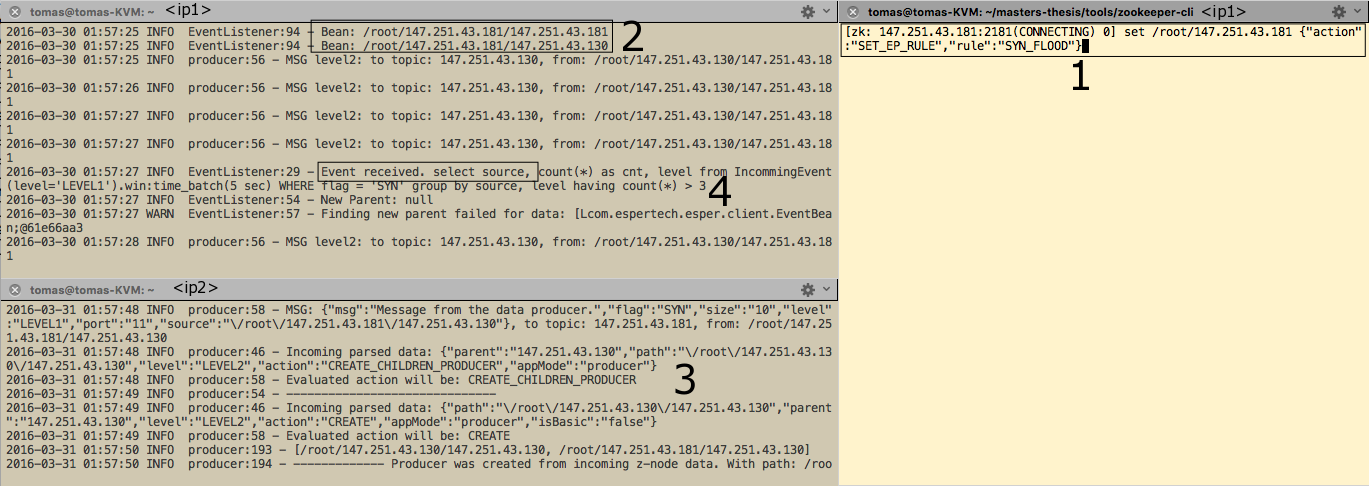
\includegraphics[width=\linewidth, height=.3\textheight]{images/deploy-rule-screen.png}
    \caption{Nasazení pravidla na hrubozrnou analýzu}
    \label{fig:deploy-rule-screen}
\end{figure}

Druhý snímek na obrázku \ref{fig:match-pattern-screen} ukazuje detekování vzoru při jemnozrné analýze. Je vidět, že během pěti vteřin, ve kterých Esper analyzoval příchozí událostí bylo detekováno osm výskytů. To je více než minimální hranice sedm událostí, kterou specifikuje pravidlo. Jednoduše řečeno, útok \textit{syn flood} je potvrzen.

\begin{figure}[H]
	\centering
    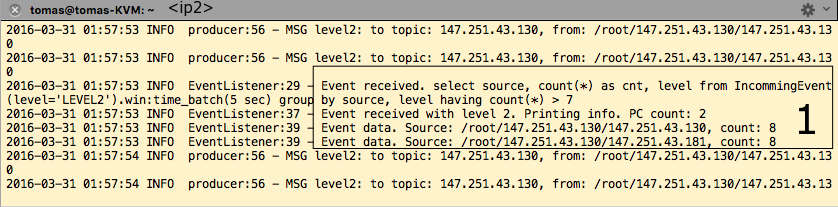
\includegraphics[width=.9\linewidth, height=.15\textheight]{images/match-pattern-screen.png}
    \caption{Detekce vzoru při jemnozrné analýze}
    \label{fig:match-pattern-screen}
\end{figure}

Na posledním snímku \ref{fig:clean-up-screen} je vidět postupné zastavování jemnozrné analýzy na počítači \textit{<ip2>}. Tím se DEM vrací do výchozího stavu z obrázku \ref{fig:kafka-impl}. Odshora jsou označeny:

\begin{enumerate}
  \item zastavení vlákna producenta
  \item smazání uzlu v ZooKeeper stromu
  \item zastavení vlákna konzumenta
\end{enumerate}

\begin{figure}[H]
	\centering
    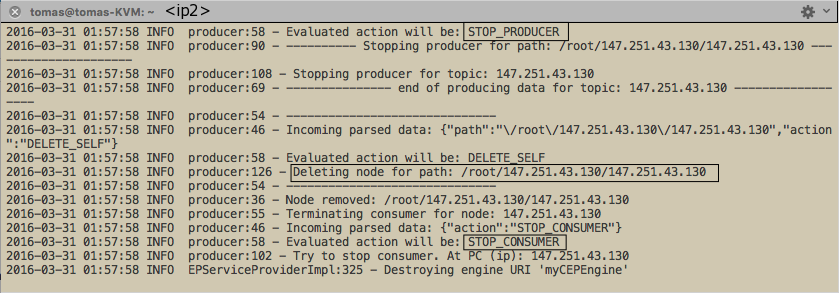
\includegraphics[width=.8\linewidth, height=.15\textheight]{images/clean-up-screen.png}
    \caption{Postupné zastavování jemnozrné analýzy}
    \label{fig:clean-up-screen}
\end{figure}

\section{Známá omezení}
Pomocí navrhovaného řešení je možné analyzovat širokou škálu událostí. Nejen dopady síťové komunikace, ale i síťový provoz jako takový. Dále je možné řešení nasadit například na analýzu aplikačních logů.

Během testování jsem narazil na některá omezení, nedostatky nebo doporučení, která v této kapitole rozvedu. K některým situacím uvedu i konkrétní řešení. U některých je řešení předmětem dalšího rozvoje algoritmu nebo jeho podrobení výkonnostním testům.

Nejdříve uvedu kompletní seznam. Každému bodu je následně věnován odstavec s popisem.

\begin{itemize}
	\item Momentální nemožnost spustit více konzumentů na jednom stroji (Více konzumentů).
	\item Monitoring a spouštění jednotlivých uzlů (Monitoring).
	\item Dynamické přidávání nových uzlů do hierarchie (Přidávání uzlů).
	\item Výpadky některých uzlů. Zookeeper je na to připraven, Kafka také, ale není jasné do jakého stavu se dostane stromová hierarchie ZooKeeperu (Výpadky).
\end{itemize}

\subsection*{Více konzumentů}
Tím, že témata v Kafce jsou členěna podle ip adres počítačů, není možné mít na jenom stroji více než jednoho konzumenta. Kdyby to tak bylo, četli by oba ze stejného tématu a "kradli si zprávy". Teoreticky by bylo možné aby se konzumenti dívali na obsah zpráv a podle toho je posílali do některé z instancí Esperu, ale takové řešení je příliš náchylné k chybám a těžko se škáluje.

Vhodným řešením by bylo přidat ke každému tématu i přepážky, které by rozlišovaly druh zpráv. V případě této práce by v každém tématu byly dvě přepážky. Jedna pro jemnozrné (\textit{LEVEL2}) a druhá pro hrubozrné události (\textit{LEVEL1}). Přepážky je možné dynamicky přidávat a tím mít možnost na jednom stroji analyzovat události množství různých typů.

\subsection*{Monitoring}
Pokud by algoritmus nasazen do produkčního prostředí, byl by zároveň potřeba zavést  důsledný monitoring. Nejen to, jestli všechny instance pracují správně, ale také jaká pravidla jsou aktuálně nasazena a na jakých strojích. Dále vytížení Kafky. Objemy zpracovávaných dat. Atd.

\subsection*{Přidávání uzlů}
Uvažoval jsem nad tím, jak by se dalo do systému dynamicky přidávat další stroje. Celá architektura je na to připravená. Jediný problém je u ZooKeeperu. Jeho konfigurace je statická a zároveň se seznam adres předává i jako vstupní parametr při startu aplikace. Před verzí \textit{3.5.0} bylo jedinou možností napsat skript, který bude postupně provádět rekonfiguraci. Od verze \textit{3.5.0} má ZooKeeper v dokumentaci [\ref{bib_7}] popsán mechanizmus pro dynamickou rekonfiguraci\footnote{Konkrétní část dokumentace: \\
https://zookeeper.apache.org/doc/trunk/zookeeperReconfig.html}.

\subsection*{Výpadky}
V rámci testování jsem zkoušel jak se aplikace vzpamatuje z výpadků některých uzlů. Chování nebylo příliš predikovatelné. Záleželo na tom v jaké fázi analýzy došlo k výpadku. Jestli byla spuštěna jemnozrná analýza nebo nikoliv. Pravidelně se opakovaly dva problémy. V ZooKeeperu zůstal zaregistrovaný některý z posluchačů a při obnově se stal znovu aktivním a tím docházelo k duplicitnímu zpracování řídících akcí. Druhým problémem byly nesmazané uzly ze ZooKeeper stromu, který se používá jako reprezentace stavu DEM.

\chapter{Závěr}
TODO - dopsat

%%Závěr bude v tomto případě obsahovat obšírnější zhodnocení toho jak se povedlo splnit zadání. Že výsledkem práce je navržené řešení za použití kafky, zk, esperu, Javy.


\begin{thebibliography}{99}
\bibitem
CCeleda, Pavel. Network Traffic Analysis for Cyber Security. Brno, 2013. Masaryk Univerzity. [online]. Dostupné z: \url{https://is.muni.cz/do/rect/habilitace/1433/44368572/44368651/HP_kor.-verejna.pdf} \label{bib_celeda}

\bibitem
LLUCKHAM, David. \textit{The Power of Events: An Introduction to Complex
Event Processing in Distributed Enterprise Systems.} Addison-Wesley Professional, 2002. ISBN 978-0-201-72789-0. \label{bib_1}

\bibitem
CCOULOURIS, George F. \textit{Distributed systems: concepts and design}. 5th ed. Boston: Addison-Wesley, c2012. ISBN 01-321-4301-1. \label{bib_2}
%% Dostupné z: \url{https://azmuri.files.wordpress.com/2013/09/george-coulouris-distributed-systems-concepts-and-design-5th-edition.pdf}

\bibitem
KKAMBURUGAMUVE, Supun; FOX, Geoffrey; LEAKE, David and QIU, Judy. \textit{Survey of Distributed Stream Processing for Large Stream Sources}. Technical report, 2013. [online]. Dostupné z: \url{http://grids.ucs.indiana.edu/ptliupages/publications/survey_stream_processing.pdf} \label{bib_3}

\bibitem
AApache Maven [online]. Dostupné z: \url{http://maven.apache.org} \label{bib_4}

\bibitem
AApache Kafka [online]. Dostupné z: \url{http://kafka.apache.org} \label{bib_5}

\bibitem
OOfficial Google documentation  [online]. Dostupné z: \url{https://support.google.com/analytics/answer/1662518?hl=en&ref_topic=3205717} \label{bib_6}

\bibitem
AApache ZooKeeper [online]. Dostupné z: \url{https://zookeeper.apache.org/} \label{bib_7}

\bibitem
GGAMMA, Erich, Richard HELM, Ralph JOHNSON a John VLISSIDES. GANG OF FOUR. \textit{Design Patterns: Elements of Reusable Object-Oriented Software}. Addison-Wesley, 1994. ISBN 0-201-63361-2 \label{bib_8}

\bibitem
AApache Curator [online]. Dostupné z: \url{http://curator.apache.org/index.html} \label{bib_9}

\bibitem
PProcess real-time big data with Twitter Storm [online]. Dostupné z: \url{http://www.ibm.com/developerworks/library/os-twitterstorm/} \label{bib_distributed_computing}



\end{thebibliography}
\appendix %% Start the appendices.

\end{document}
